\chapter{ĐỘNG LƯỢNG}
\setcounter{section}{17}
\section{ĐỘNG LƯỢNG VÀ ĐỊNH LUẬT BẢO TOÀN ĐỘNG LƯỢNG}
\subsection{Tóm tắt lí thuyết}
\begin{tomtat}
	\subsubsection{Động lượng}
	\begin{dn}
		Động lượng là đại lượng đặc trưng cho khả năng \textbf{truyền chuyển động} của vật này lên vật khác thông qua tương tác giữa chúng.\\
		Động lượng của một vật được xác định bằng tích của khối lượng và vận tốc của vật:
	\begin{equation}
		\vec{p}=m\cdot\vec{v}\\
		\label{eq:1}
	\end{equation}
		\end{dn}
	Trong đó:
	\begin{itemize}
		\item $\vec{p}$: động lượng của vật, đơn vị trong hệ SI là \si{\kilogram\cdot\meter/\second};
		\item $m$: khối lượng của vật, đơn vị trong hệ SI là \si{\kilogram};
		\item $\vec{v}$: vận tốc của vật, đơn vị trong hệ SI là \si{\meter/\second}.
	\end{itemize}
	\begin{note} \textbf{Lưu ý:}
	\begin{itemize}
		\item Động lượng là đại lượng vector có hướng cùng với hướng của vận tốc;
		\item Động lượng phụ thuộc vào hệ quy chiếu;
		\item Vector động lượng của hệ vật bằng tổng các vector động lượng của các vật trong hệ.
	\end{itemize}
	\end{note}
	\subsubsection{Định luật bảo toàn động lượng}
	\paragraph{Khái niệm hệ kín}
	\begin{dn}
		Một hệ được xem là \textbf{hệ kín} khi hệ đó không có tương tác với các vật bên ngoài hệ.\\
		Ngoài ra, khi tương tác của các vật bên ngoài hệ (ngoại lực) lên hệ \textbf{\textit{bị triệt tiêu}} hoặc \textbf{\textit{không đáng kể}} so với tương tác giữa các thành phần của hệ (nội lực), hệ vẫn có thể được xem \textbf{\textit{gần đúng là hệ kín}}.
	\end{dn}
	\textbf{\textit{Ví dụ:}}
	\dongcham{8}
	\paragraph{Định luật bảo toàn động lượng}
	\begin{dl}
		Động lượng của một hệ kín luôn bảo toàn:
		\begin{equation}
			\vec{p}_1+\vec{p}_2+\dots+\vec{p}_n=\vec{p}^\prime_1+\vec{p}^\prime_2+\dots+\vec{p}^\prime_n\\
			\label{eq:2}
		\end{equation}
	\end{dl}
	Trong đó:
	\begin{itemize}
		\item $\vec{p}_1+\vec{p}_2+\dots+\vec{p}_n$: tổng động lượng của các vật (trong hệ kín) trước tương tác;
		\item $\vec{p}^\prime_1+\vec{p}^\prime_2+\dots+\vec{p}^\prime_n$: tổng động lượng của các vật (trong hệ kín) sau tương tác.
	\end{itemize}
\end{tomtat}
\begin{note}
	Nếu $\sum\vec{F}\neq \vec{0}$ nhưng hình chiếu của các ngoại lực trên một phương nào đó triệt tiêu thì động của hệ bảo toàn trên phương đó.
\end{note}
\begin{dang}{Vận dụng biểu thức xác định động lượng}
	Động lượng của vật khối lượng $m$ chuyển động với vận tốc $\vec{v}$:
	$$\vec{p}=m\vec{v}.$$
\end{dang}
\begin{vd}
	Tính độ lớn động lượng trong các trường hợp sau:
	\begin{enumerate}[label=\alph*)]
		\item Một xe ô tô có khối lượng \SI{1.2}{\text{tấn}} đang chuyển động với tốc độ \SI{54}{\kilo\meter/\hour}.
		\item Một quả bóng khối lượng \SI{400}{\gram} đang bay với tốc độ \SI{20}{\meter/\second}.
		\item Một electron khối lượng \SI{9.1E-31}{\kilogram} đang chuyển động với tốc độ \SI{2.5E6}{\meter/\second}.
	\end{enumerate}
\end{vd}
\begin{vd}
	Một ô tô khối lượng \SI{1}{\text{tấn}} khởi hành từ trạng thái nghỉ có gia tốc không đổi là \SI{1}{\meter/\second^2}. Tính động lượng của ô tô sau khi nó đi được quãng đường \SI{50}{\meter}.
\end{vd}
\begin{vd}
	Một quả bóng có khối lượng $m=\SI{0.2}{\kilogram}$ đập vuông góc vào tường với tốc độ $v_1=\SI{5}{\meter/\second}$ và bật ngược trở lại với tốc độ $v_2=\SI{4}{\meter/\second}$. Tính độ biến thiên động lượng của quả bóng.
\end{vd}
\begin{dang}{Xác định động lượng của hệ vật}
	Động lượng của hệ vật tương tác bằng tổng động lượng của các vật thành phần:
	$$\vec{p}=\vec{p}_1+\vec{p}_2+\dots+\vec{p}_n.$$
	Để tìm vector động lượng tổng hợp, ta sử dụng quy tắc hình bình hành (hoặc tam giác vector):
	$$\vec{p}=\vec{p}_1+\vec{p}_2\Rightarrow p=\sqrt{p^2_1+p^2_2+2p_1p_2\cos\alpha}.$$
	\begin{center}
		\begin{tabular}{M{6cm}M{2cm}M{6cm}}
				\begin{tikzpicture}
				\coordinate(O) at (0,0);
				\coordinate(A) at ($(O)+(60:3)$);
				\coordinate(B) at ($(O)+(5.5,0)$);
				\coordinate(A1) at ($(B)+(-120:3)$);
				\draw[-stealth, blue, line width=1.5pt] (O)--(A);
				\draw[dashed, line width=1pt] (A)--(B);
				\draw[dashed, line width=1pt] (A1)--(B);
				\draw[-stealth, orange, line width=1.5pt] (O)--(A1);
				\draw[-stealth, teal, line width=1.5pt] (O)--(B);
				\node[left,blue] at ($(O)!0.5!(A)$) {$\vec{p}_1$};
				\node[below,orange] at ($(A1)!0.5!(B)+(0.2,0)$) {$\vec{p}_2$};
				\node[below,teal] at ($(O)!0.5!(B)$) {$\vec{p}$};
				\tkzMarkAngle[size=0.75cm,color=black](A1,O,A);
				\tkzLabelAngle[color=black,pos=1.2](A1,O,A){$\alpha$};
			\end{tikzpicture} 
			&&
			\begin{tikzpicture}
				\coordinate(O) at (0,0);
				\coordinate(A) at ($(O)+(60:3)$);
				\coordinate(B) at ($(O)+(5.5,0)$);
				\draw[-stealth, blue, line width=1.5pt] (O)--(A);
				\draw[-stealth, orange, line width=1.5pt] (A)--(B);
				\draw[-stealth, teal, line width=1.5pt] (O)--(B);
				\node[left,blue] at ($(O)!0.5!(A)$) {$\vec{p}_1$};
				\node[right,orange] at ($(A)!0.5!(B)+(0.2,0)$) {$\vec{p}_2$};
				\node[below,teal] at ($(O)!0.5!(B)$) {$\vec{p}$};
			\end{tikzpicture} 
		\end{tabular}
	\end{center}
	\textbf{Các trường hợp riêng:}
	\begin{center}
		\begin{tabular}{M{5.5cm}M{5.5cm}M{6cm}}
			\textbf{* Trường hợp $\vec{p}_{1}\uparrow\uparrow\vec{p}_{2}$}&\textbf{* Trường hợp $\vec{p}_{1}\uparrow\downarrow\vec{p}_{2}$}&\textbf{* Trường hợp $\vec{p}_{1}\bot\vec{p}_{2}$}\\
			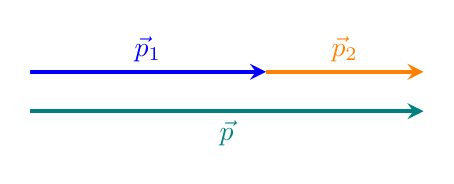
\begin{tikzpicture}
				\draw[-stealth, blue, line width=1.5pt] (0,0)--(3,0);
				\draw[-stealth, orange, line width=1.5pt] (3,0)--(5,0);
				\draw[-stealth, teal, line width=1.5pt] (0,-0.5)--(5,-0.5);
				\node[above, blue] at (1.5,0) {$\vec{p}_{1}$};
				\node[above, orange] at (4,0) {$\vec{p}_{2}$};
				\node[below, teal] at (2.5,-0.5) {$\vec{p}$};
			\end{tikzpicture}&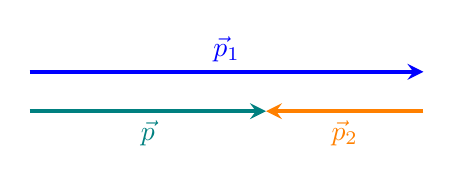
\begin{tikzpicture}
				\draw[-stealth, blue, line width=1.5pt] (0,0)--(5,0);
				\draw[-stealth, orange, line width=1.5pt] (5,-0.5)--(3,-0.5);
				\draw[-stealth, teal, line width=1.5pt] (0,-0.5)--(3,-0.5);
				\node[above, blue] at (2.5,0) {$\vec{p}_{1}$};
				\node[below, orange] at (4,-0.5) {$\vec{p}_{2}$};
				\node[below, teal] at (1.5,-0.5) {$\vec{p}$};
			\end{tikzpicture}&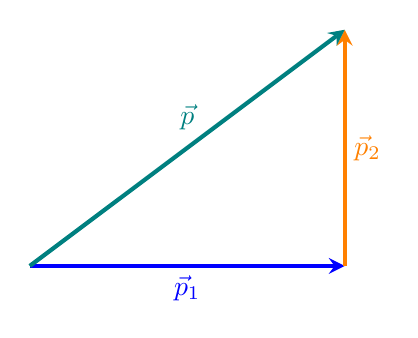
\begin{tikzpicture}
				\draw[-stealth, blue, line width=1.5pt] (0,0)--(4,0);
				\draw[-stealth, orange, line width=1.5pt] (4,0)--(4,3);
				\draw[-stealth, teal, line width=1.5pt] (0,0)--(4,3);
				\node[below, blue] at (2,0) {$\vec{p}_{1}$};
				\node[right, orange] at (4,1.5) {$\vec{p}_{2}$};
				\node[above, teal] at (2,1.6) {$\vec{p}$};
			\end{tikzpicture}\\
			$p=p_{1}+p_{2}$&$p=\left|p_{1}-p_{2}\right|$&$p^2=p^2_{1}+p^2_{2}$
		\end{tabular}
		
	\end{center}
	\begin{note}
		Trường hợp $p_1=p_2$ và $\left(\vec{p}_1,\vec{p}_2\right)=\alpha$ thì $p=2p_1\cos\dfrac{\alpha}{2}$.
	\end{note}
\end{dang}
\begin{vd}
	Tìm động lượng (hướng và độ lớn) của hệ hai vật $m_1=\SI{3}{\kilogram}$, $m_2=\SI{4}{\kilogram}$, $v_1=v_2=\SI{2}{\meter/\second}$. Biết hai vật chuyển động theo các hướng:
	\begin{enumerate}[label=\alph*)]
		\item ngược nhau.
		\item vuông góc nhau.
		\item hợp với nhau góc \SI{60}{\degree}.
	\end{enumerate}
\end{vd}
\begin{dang}{Bài toán tương tác giữa hai vật trong hệ kín}
	Động lượng của hệ kín (hệ cô lập) luôn bảo toàn:
	\begin{equation}
		\vec{p}_1+\vec{p}_2=\vec{p}^\prime_1+\vec{p}^\prime_2\\
		\label{eq:3}
	\end{equation}
	Tương tự khi làm việc với các đại lượng vector như lực hay vận tốc, để giải phương trình \eqref{eq:3} thông thường ta sẽ gặp 2 trường hợp sau:
	\begin{itemize}
		\item \textbf{Trường hợp 1:} Các vector động lượng cùng phương.\\
		Ta chọn chiều dương rồi chiếu phương trình \eqref{eq:3} lên chiều dương.
		\item  \textbf{Trường hợp 2:} Các vector động lượng khác phương.\\
		Ta dựng tam giác vector, dùng định lý hàm $\sin$ hoặc cosin để giải.
	\end{itemize}
	
\end{dang}
\begin{vd}
	Một ô tô con khối lượng \SI{1.2}{\text{tấn}} đang chuyển động với tốc độ \SI{25}{\meter/\second} thì va chạm vào đuôi của một xe tải khối lượng \SI{9}{\text{tấn}} đang chạy cùng chiều với tốc độ \SI{20}{\meter/\second}. Sau va chạm, ô tô con vẫn chuyển động theo hướng cũ với tốc độ \SI{18}{\meter/\second}.
	\begin{center}
		\includegraphics[scale=0.5]{figs/DONGLUONG-2}
	\end{center}
	\begin{enumerate}[label=\alph*)]
		\item Xác định vận tốc của xe tải ngay sau va chạm.
		\item  Xác định phần năng lượng tiêu hao trong quá trình va chạm. Giải thích tại sao lại có sự tiêu hao năng lượng này.
	\end{enumerate}
\end{vd}
\begin{vd}
	Một toa xe có khối lượng 4 tấn chuyển động đến va chạm vào toa xe thứ hai đang đứng yên. Sau va chạm, cả hai cùng chuyển động với vận tốc \SI{2}{\meter/\second}. Hỏi toa xe thứ nhất có vận tốc là bao nhiêu trước khi móc vào toa xe thứ hai? Cho biết toa xe thứ hai có khối lượng 2 tấn.
\end{vd}
\begin{vd}
	Một viên đạn đang bay theo phương ngang với vận tốc \SI{200}{\meter/\second} thì nổ thành hai mảnh có khối lượng \SI{10}{\kilogram} và \SI{5}{\kilogram}. Mảnh  nhỏ bay lên trên theo phương thẳng đứng với tốc độ \SI{346}{\meter/\second}. Hỏi mảnh to bay theo phương nào, với vận tốc bằng bao nhiêu? Bỏ qua sức cản không khí.
\end{vd}
\begin{dang}{Bài toán chuyển động bằng phản lực}
	\begin{dn}
		Chuyển động bằng phản lực là loại chuyển động do tương tác bên trong nên một phần của vật tách rời khỏi vật chuyển động về một hướng và phần còn lại chuyển động theo hướng ngược lại.
	\end{dn}
	\textbf{\textit{Ví dụ:}}
	\begin{itemize}
		\item Chuyển động của tên lửa.
		\item Chuyển động giật lùi của súng khi bắn.
	\end{itemize}
	\begin{note}
		Trong các bài toán đạn nổ, bắn súng, phóng tên lửa thì nội lực trong hệ là rất lớn so với ngoại lực tác dụng lên hệ. Do đó, ta có thể xem các hệ nói trên gần đúng là hệ kín.
	\end{note}
	Xét khẩu súng có khối lượng $m_\mathrm{s}$ và viên đạn có khối lượng $m_{\text{đ}}$ ban đầu đứng yên. Sau đó, bóp cò để viên đạn bắn khỏi nòng với vận tốc $\vec{v}_{\text{đ}}$. Gọi $\vec{v}_{\mathrm{s}}$ là vận tốc của súng sau khi viên đạn được bắn ra.
	\begin{center}
		\includegraphics[scale=0.25]{figs/DONGLUONG-3}
	\end{center}
	Áp dụng định luật bảo toàn động lượng cho hệ súng - đạn ngay trước và sau khi bắn:
	\begin{eqnarray*}
		&&\vec{0}=\vec{p}_{\text{đ}}+\vec{p}_{\mathrm{s}}\\
		&\Leftrightarrow& \vec{0}=m_{\text{đ}}\vec{v}_{\text{đ}}+m_{\text{s}}\vec{v}_{\text{s}}\\
		&\Rightarrow& \vec{v}_{s}=-\dfrac{m_{\text{đ}}}{m_{\text{s}}}\cdot\vec{v}_{\text{đ}}
	\end{eqnarray*}
Dấu $"-"$ thể hiện súng bị giật lùi trở lại. Tốc độ giật lùi của súng là $v_{\mathrm{s}}=\dfrac{m_{\text{đ}}}{m_{\text{s}}}\cdot v_{\text{đ}}$.
\end{dang}
\begin{vd}
Xạ thủ Nguyễn Minh Châu là người giành huy chương vàng ở nội dung \SI{10}{\meter} súng ngắn hơi nữ ngay lần đầu tham dự SEA Games 27. Khẩu súng chị sử dụng nặng \SI{1.45}{\kilogram} với viên đạn nặng \SI{7.4}{\gram}. Tốc độ đạn khi rời khỏi nòng là \SI{660}{fps} $\left(\SI{1}{fps}=\SI{0.3}{\meter/\second}\right)$. Hỏi khi bắn, nòng súng giật lùi với tốc độ bao nhiêu?
\end{vd}
\begin{vd}Một nữ phi hành gia khi đang thực hiện nhiệm vụ tại một vị trí cách cửa trạm không gian một đoạn \SI{140}{\meter} thì sợi dây kết nối cô với trạm đột ngột bị đứt. 
	\immini{Để có thể quay trở lại, từ trạng thái cân bằng, phi hành gia đã gỡ và ném bình oxygen với tốc độ \SI{5}{\meter/\second} theo hướng ra xa trạm không gian. Biết tổng khối lượng của phi hành gia và toàn bộ thiết bị hỗ trợ (kể cả bình oxygen) là \SI{82}{\kilogram}, khối lượng bình oxygen là \SI{12}{\kilogram} và lượng khí trong mũ bảo hiểm đủ để cô ấy có thể duy trì hô hấp thông thường trong \SI{3}{\minute}. Hỏi phi hành gia có thể quay trở về trạm an toàn không?}
	{\includegraphics[scale=0.4]{figs/DONGLUONG-4}}
\end{vd}
\begin{dang}{Bài toán liên quan đến chuyển động tổng hợp}
	\textbf{\textit{Nhắc lại công thức vận tốc tổng hợp:}}
	$$\vec{v}_{13}=\vec{v}_{12}+\vec{v}_{23}.$$
	\textbf{BÀI TOÁN KHẢO SÁT}\\
	Tên lửa khối lượng $M$ đang bay với vận tốc $\vec{v}_0$ thì phụt ra lượng khí khối lượng $m$ với vận tốc $\vec{v}_{\mathrm{k}}$ về phía sau \textbf{so với tên lửa}. Tốc độ của tên lửa sau khi phụt khí bằng bao nhiêu?\\
\immini{	Chọn hệ quy chiếu gắn với đất.\\
	Gọi:
	\begin{itemize}
		\item (1) khí;
		\item (2) tên lửa;
		\item (0) mặt đất.
\end{itemize}}{\includegraphics[scale=0.35]{figs/DONGLUONG-5}\\}
	Như vậy: $\vec{v}_{20}=\vec{v}_0$; $\vec{v}^\prime_{12}=\vec{v}_{\mathrm{k}}$; $\vec{v}^\prime_{20}=\vec{v}=?$.
	\begin{center}
		\begin{tabular}{|M{5cm}|M{5cm}|M{5cm}|}
			\hline
			&\thead{Tên lửa}& \thead{Khí}\\
			\hline
			\thead{Động lượng ban đầu} & $M\cdot\vec{v}_{20}$& $\vec{0}$\\
			\hline
			\thead{Động lượng lúc sau} & $\left(M-m\right)\cdot\vec{v}^\prime_{20}$& $m\cdot\vec{v}^\prime_{10}$\\
			\hline
		\end{tabular}
	\end{center}
	Áp dụng định luật bảo toàn động lượng cho hệ tên lửa - khí ngay trước và sau khi phụt khí:
	\begin{eqnarray*}
		&&M\cdot\vec{v}_{20}=\left(M-m\right)\cdot\vec{v}^\prime_{20}+m\cdot\vec{v}^\prime_{10}\\
		&\Leftrightarrow&M\cdot\vec{v}_{20}=\left(M-m\right)\cdot\vec{v}^\prime_{20}+m\cdot\left(\vec{v}^\prime_{12}+\vec{v}^\prime_{20}\right)\\
		&\Leftrightarrow&M\cdot\vec{v}_{0}=\left(M-m\right)\cdot\vec{v}+m\cdot\left(\vec{v}_{\mathrm{k}}+\vec{v}\right)\\
		&\Leftrightarrow&M\cdot\vec{v}_{0}=M\cdot\vec{v}+m\cdot\vec{v}_{\mathrm{k}}\\
	\end{eqnarray*}
	Chọn chiều dương là chiều chuyển động ban đầu của tên lửa:
	$$Mv_0=Mv-mv_{\mathrm{k}}\Rightarrow v=\dfrac{Mv_0+mv_k}{M}.$$
\end{dang}
\begin{vd}
	Tên lửa khối lượng tổng cộng 100 tấn đang bay với tốc độ \SI{200}{\meter/\second} thì phụt tức thời ra 20 tấn khí về phía sau với tốc độ \SI{500}{\meter/\second} so với tên lửa. Tìm vận tốc của tên lửa sau khi phụt khí nếu bỏ qua lực hấp dẫn của Trái Đất và lực cản của không khí.
\end{vd}